\subsection{Mechanism design}
Now we established all formulas and theories for 2D, 3D and nD-Laplace we are being able to give a full design of the mechanism.

\begin{figure}[H]
    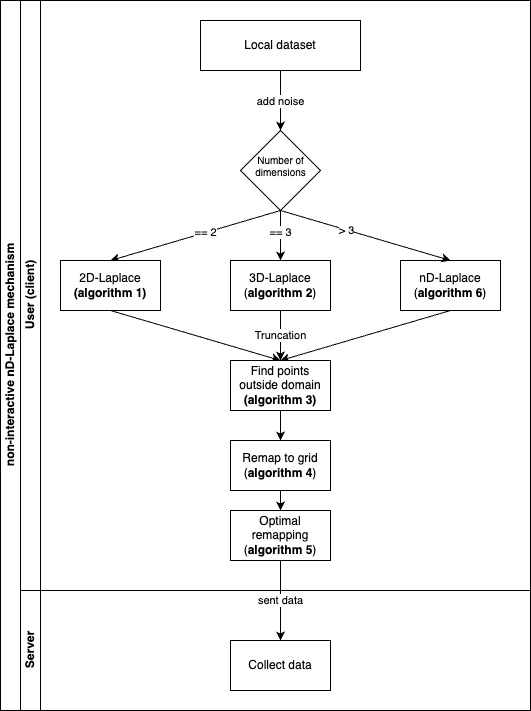
\includegraphics[width=0.6\textwidth]{TheorethicalFramework/ND-Laplace/Images/final_mechanism_design.png}
    \caption{Non-interactive mechanism design for nD-Laplace.}
    \label{fig:final-mechanism-design}
\end{figure}

For easy navigation, we provide a list of all algorithms:
\begin{enumerate}
    \item 2D-Laplace:  \ref{alg:2d-laplace}
    \item 3D-Laplace: \ref{alg:3d-laplace}
    \item nD-Laplace: \ref{alg:nd-laplace}
    \item Find points outside domain: \ref{alg:find-outside-domain-laplace}
    \item Grid remapping: \ref{alg:grid-remapping-laplace}
    \item Optimal remapping: \ref{alg:optimal-remapping-laplace}
\end{enumerate}
\newpage
\subsubsection{Practical example}
The shape of the dataset is important for the usefulness of clustering.
With our algorithm, there are four different shapes/variants of the dataset.
To provide an example, this has been visualized using a 3D dataset based on the Cardiotocography dataset (\ref{datasets-section}).
The goal for our mechanism is to provide privacy, but also to preserve the shape of the dataset to benefit the utility of clustering.
Grid remapping and ultimately optimal remapping are used to achieve this goal.

\begin{figure}[H]
    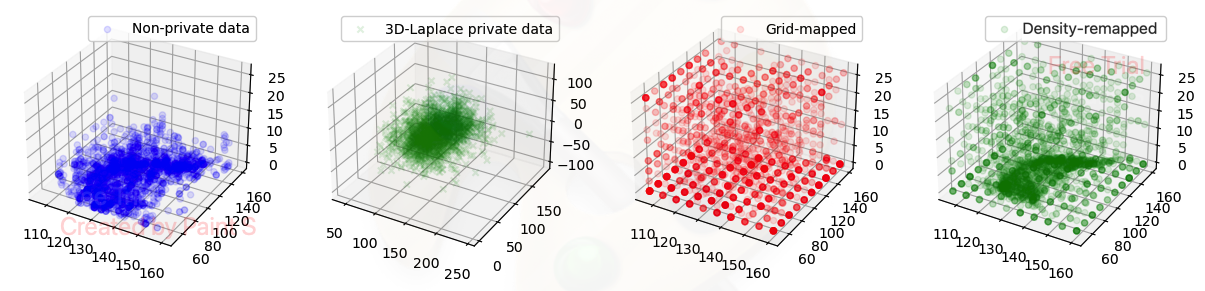
\includegraphics[width=1.1\textwidth]{TheorethicalFramework/ND-Laplace/Images/optimal-remapping-example.png}
    \caption{Example of optimal remapping for the 3D-dataset: Cardiotocography. The example shows the different steps of the mechanism in sequence for a dataset perturbed with a privacy budget of 0.1.}
\end{figure}

\todo[inline]{Explain more in-depth what is happening in the example.}